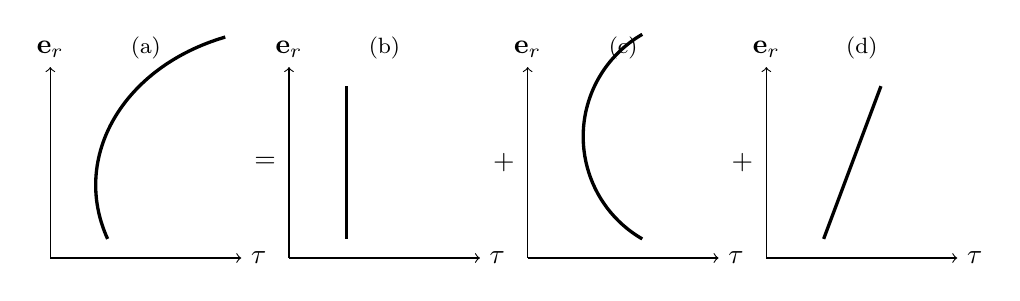
\begin{tikzpicture}
	\def\len{.2*\textwidth}
	\def\spx{.2/4*\textwidth}
	
	
	\draw[->] (0,0) node (tot) {} -- ++(\len,0) node [right]{$\tau$};
	\draw[->] (tot.center) -- ++(0,\len) node [above]{$\mathbf e_r$};
	
	\draw (\len+\spx/2,\len/2) node{$=$};
	
	\draw[very thick] (.3*\len,.1*\len) arc [start angle=200, end angle=110, x radius=2.5, y radius=2];
	
	\draw (.5*\len,1.1*\len) node{\footnotesize(a)};
	
	
	\draw[->] ({\len+\spx},0) node (TA) {} -- ++(\len,0) node [right]{$\tau$};
	\draw[->] (TA.center) -- ++(0,\len) node [above]{$\mathbf e_r$};
	
	\draw ({2*\len+3*\spx/2},\len/2) node{$+$};
	
	\draw[very thick] (1.3*\len+\spx,.1*\len) -- ++(0,.8*\len);
	
	\draw (1.5*\len+\spx,1.1*\len) node{\footnotesize(b)};
	
	
	\draw[->] ({2*(\len+\spx)},0) node (Cond) {} -- ++(\len,0) node [right]{$\tau$};
	\draw[->] (Cond.center) -- ++(0,\len) node [above]{$\mathbf e_r$};
	
	\draw ({3*\len+5*\spx/2},\len/2) node{$+$};	
	
	\draw[very thick] (2.6*\len+2*\spx,.1*\len) arc [start angle=-120, end angle=-240, x radius=1.5, y radius=1.5];
	
	\draw (2.5*\len+2*\spx,1.1*\len) node{\footnotesize(c)};
	
	
	\draw[->] ({3*(\len+\spx)},0) node (Conv) {} -- ++(\len,0) node [right]{$\tau$};
	\draw[->] (Conv.center) -- ++(0,\len) node [above]{$\mathbf e_r$};
	
	\draw[very thick] (3.3*\len+3*\spx,.1*\len) -- ++(.3*\len,.8*\len);
	
	\draw (3.5*\len+3*\spx,1.1*\len) node{\footnotesize(d)};
\end{tikzpicture}